

\chapter{Materiais} \label{cap:materiais}
\vspace{-2cm}
Neste capítulo serão apresentados os materiais a serem utilizados neste projeto.\newline
%\vspace{1cm}

%%%%%%%%%%%%%%%%%%%%%%%%%%%%%%%%%%%%%%%%%%%%%%%%%%%%%%%%%%%%%%%%%%%%%%%%%%%%%%%%%%%%%%%%%%%%%%%%%%%%%%%%%%%%%%%%%
\section{Microcontrolador} \label{cap:micro}

Será utilizado o \textit{Kit} de desenvolvimento NUCLEO-F303K8, da ST Microelectronics, %\textsuperscript{TM}, 
o qual pode ser visto na Figura \ref{fig:nucleo}. Esta placa utiliza o microcontrolador STM32F303K8, que possui como processador 
ARM Cortex-M4. Este processador dispõe de uma FPU, a qual facilita o processamento dos cálculos em ponto flutuante que são 
necessários para o controle do veículo. As principais informações deste dispositivo estão na Tabela \ref{tab:micro}.

\begin{figure}[h!]
 \centering
 \captionsetup{width=0.4\textwidth,font=footnotesize,textfont=bf}
 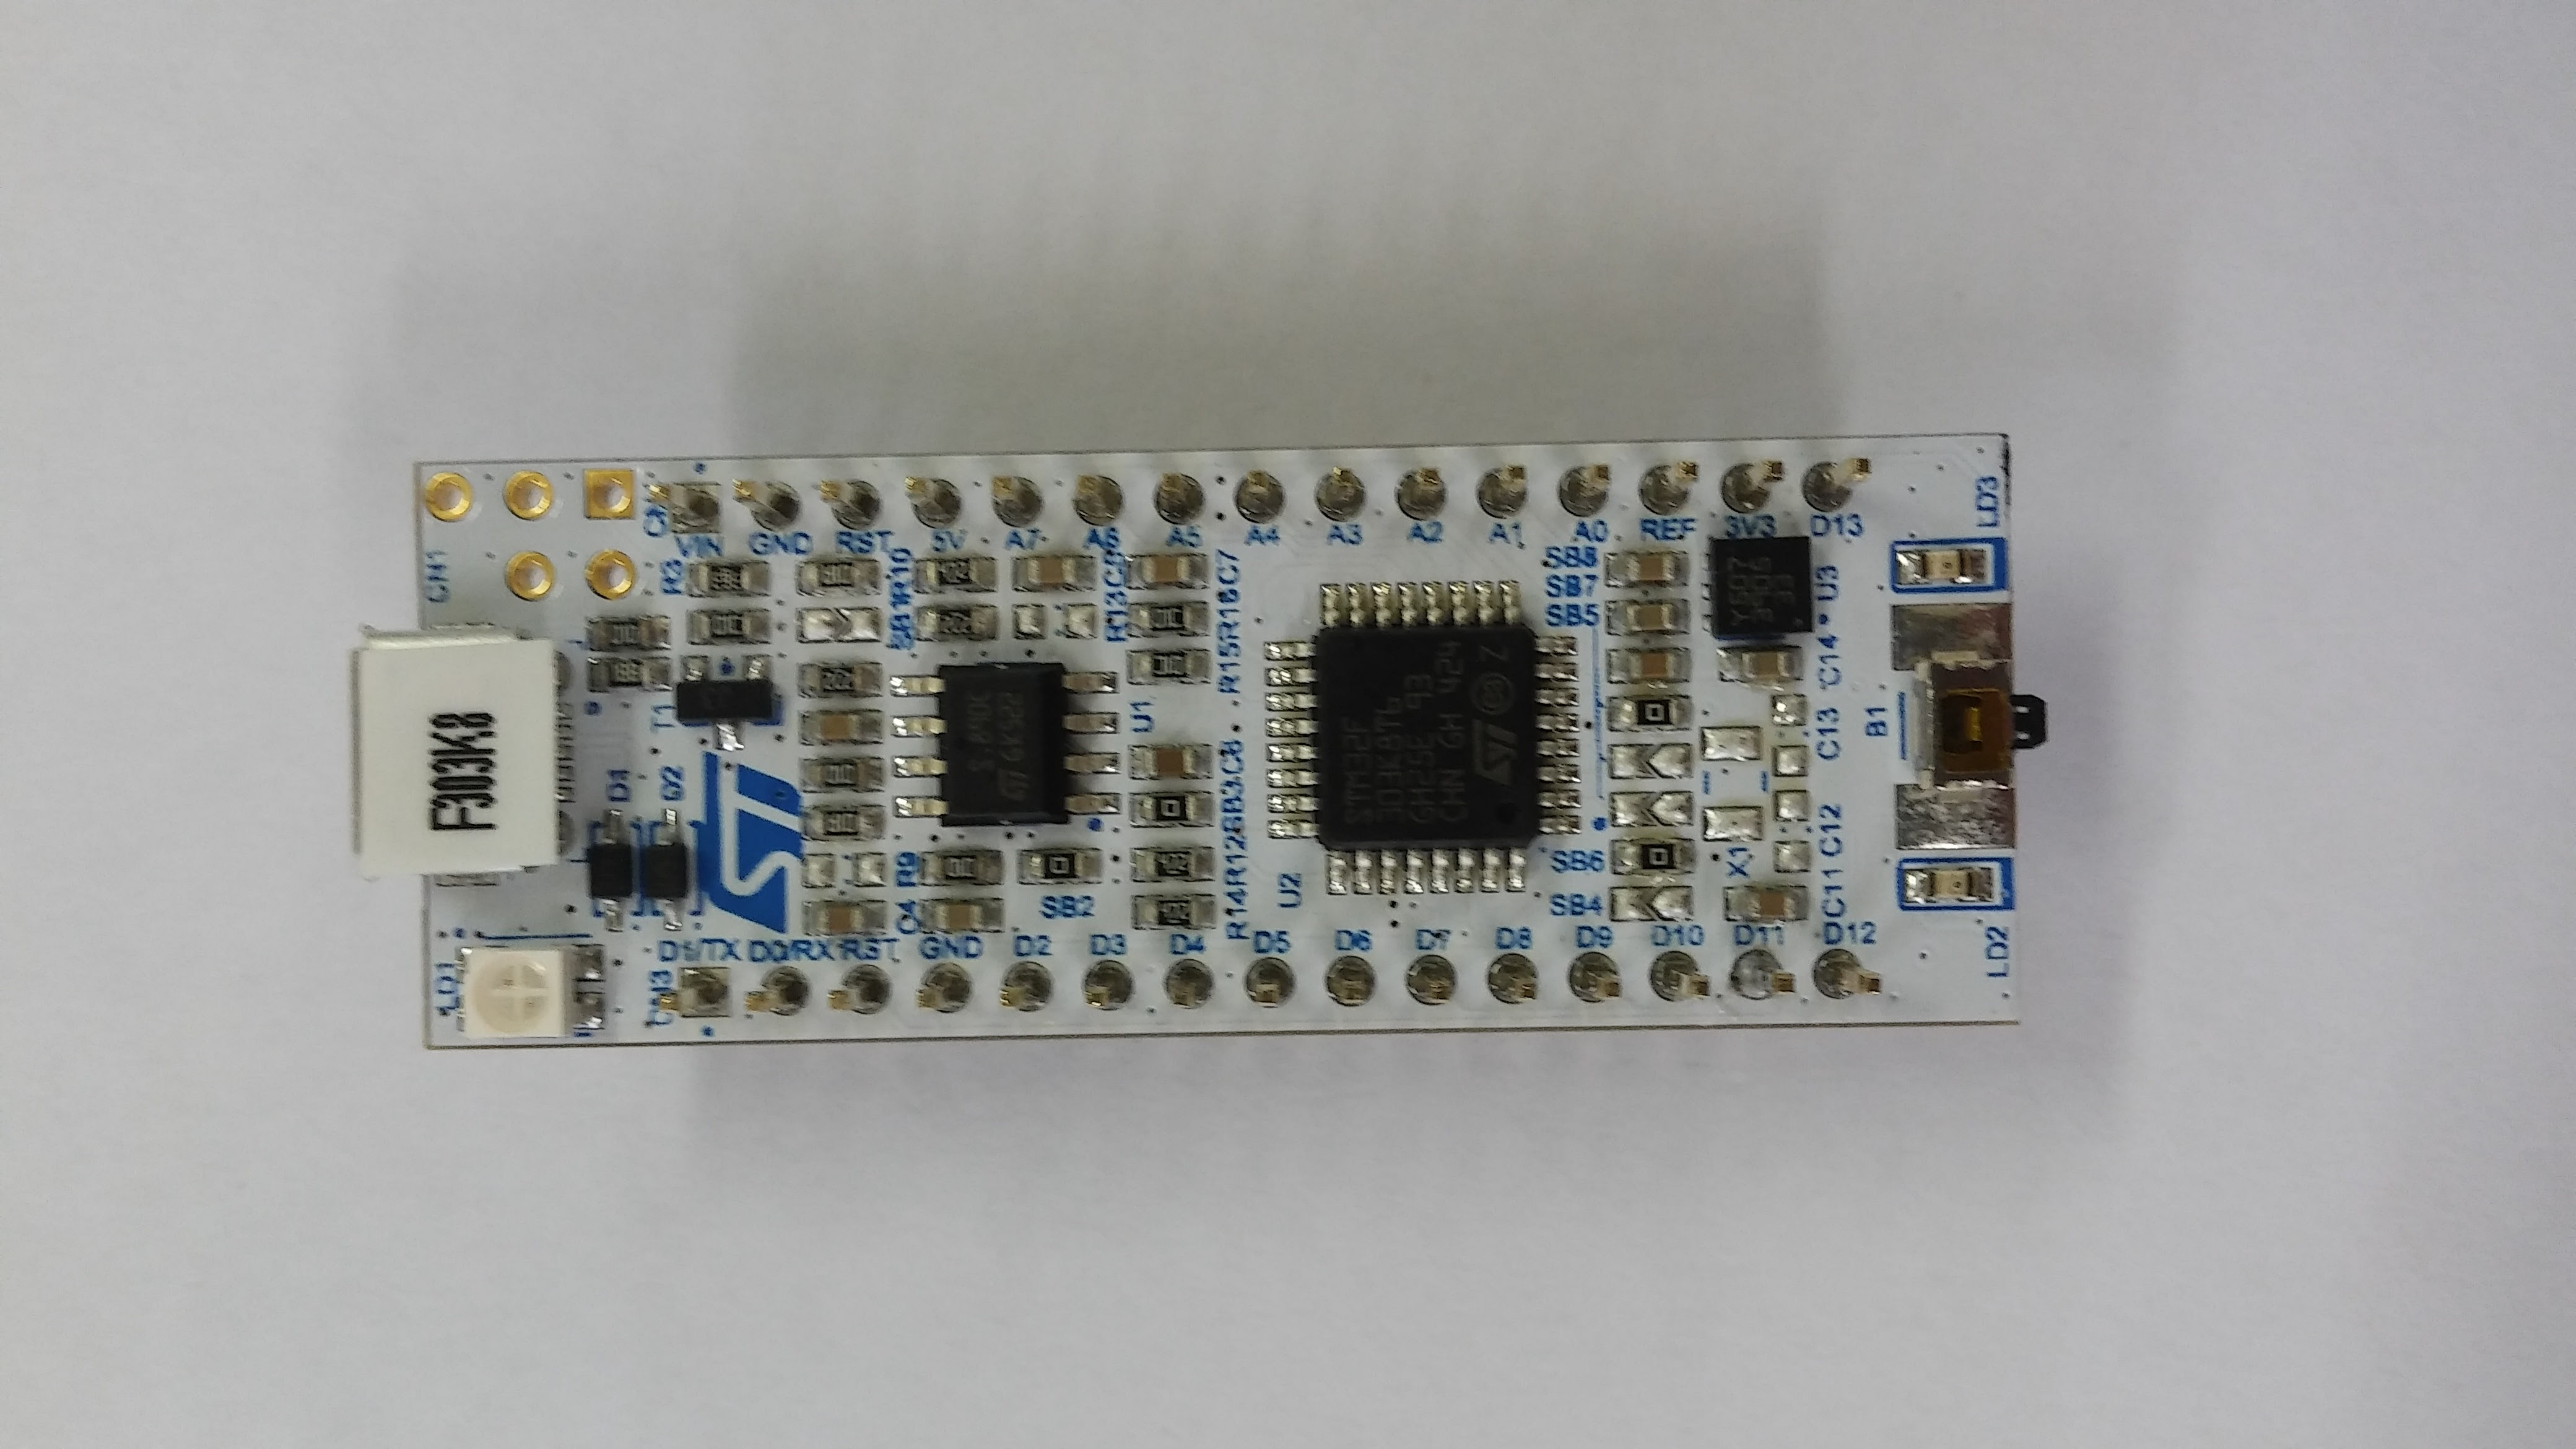
\includegraphics[width=0.4\textwidth,height=0.8\textheight,keepaspectratio]{figuras/nucleo.jpg}
 \caption{\textit{Kit} de desenvolvimento STM32-F303K8 \label{fig:nucleo}}
 \vspace{-0.3cm}
 \caption*{Fonte: Autoria própria}.
\end{figure}


\begin{table}[h!]
\centering
\captionsetup{width=0.66\textwidth,font=footnotesize,textfont=bf}
\caption{Especificações do microcontrolador STM32F303K8 \label{tab:micro}}
\begin{tabular}{llllllll}
\cline{1-2}
\bf Característica & \bf Descrição & & &  \\ \cline{1-2}
Frequência de operação & 72MHz & & &  \\
Desempenho & 90 \sigla{DMPIS}{\textit{Dhrystone Million Instructions per Second}}\protect\footnote{DMPIS é uma 
medida de desempenho para avaliar um sistema embarcado.} & & &  \\
\textit{Flash} & 64KB & & &  \\
SRAM & 16KB & & &  \\
Quantidade de temporizadores (\textit{timers}) & 11 & & &  \\
Quantidade de canais do ADC & 21 & & &  \\
Resolução do ADC & 12 \textit{bits} & & &  \\ \cline{1-2}
\end{tabular}
\vspace{0.1cm}
\caption*{Fonte: \cite{stm303} }
\end{table}


%%%%%%%%%%%%%%%%%%%%%%%%%%%%%%%%%%%%%%%%%%%%%%%%%%%%%%%%%%%%%%%%%%%%%%%%%%%%%%%%%%%%%%%%%%%%%%%%%%%%%%%%%%%%%%%
\section{Motores CC} \label{cap:motores}
Será utilizado o motor CC modelo 3041 da Pololu, %\textsuperscript{TM} 
o qual pode ser visto na Figura \ref{fig:motor}. Estes motores são classificados pela fabricante como 
\textit{High-Power Carbon Brush} (\sigla{HPCB}{\textit{High-Power Carbon Brush}}), os quais são motores 
escovados \textit{brushed}\protect\footnote{Um motor escovado realiza a troca de fase do rotor através de escovas.}. 
Este modelo possui o eixo estendido, possibilitando o acoplamento de um \textit{encoder}, a partir do qual é possível fazer o 
mapeamento da pista. 
As principais especificações técnicas deste dispositivo estão na Tabela \ref{tab:motor}.


\begin{figure}[h!]
 \centering
 \captionsetup{width=0.4\textwidth,font=footnotesize,textfont=bf}
 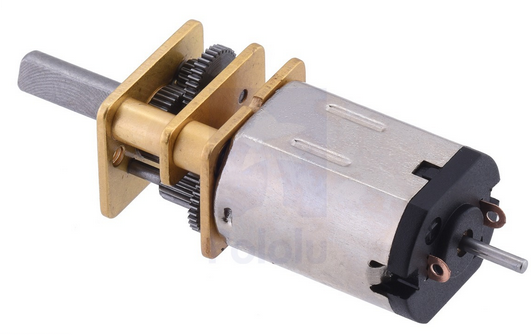
\includegraphics[width=0.4\textwidth,height=0.8\textheight,keepaspectratio]{figuras/motor.png}
 \caption{Motor HPCB 3041 \label{fig:motor}}
 \vspace{-0.3cm}
 \caption*{Fonte: \cite{pololu_motor}}.
\end{figure}


\begin{table}[h!]
\centering
\captionsetup{width=0.63\textwidth,font=footnotesize,textfont=bf}
\caption{Especificações do motor 3041 da Pololu \label{tab:motor}}
\begin{tabular}{llllllll}
\cline{1-2}
\bf Característica & \bf Descrição & & &  \\ \cline{1-2}
Tensão de alimentação & 12V & & &  \\
Corrente de alimentação (sem carga) & 100mA  & & &  \\
Corrente máxima de alimentação & 800mA & & &  \\
Caixa de velocidade & 10:1 & & &  \\
Rotação máxima & 3000 \sigla{RPM}{\textit{Revolutions Per Minute}} & & &  \\
Torque máximo & 0.3kg-cm & & &  \\ \cline{1-2}
\end{tabular}
\vspace{0.1cm}
\caption*{Fonte: \cite{pololu_motor} }
\end{table}

\vspace{0.5cm}
%%%%%%%%%%%%%%%%%%%%%%%%%%%%%%%%%%%%%%%%%%%%%%%%%%%%%%%%%%%%%%%%%%%%%%%%%%%%%%%%%%%%%%%%%%%%%%%%%%%%%%%%%%%%%%%
\section{Ponte H} \label{cap:ponteh}

Para o acionamento dos motores, será utilizada uma Ponte H, que é um circuito que tem esse nome devido à sua configuração, que 
se parece com um 'H', como pode ser visto na Figura \ref{fig:ponte}. A Ponte H controla não só a velocidade entregue aos motores, mas 
também o seu sentido.
O modelo que será utilizado é o TB6612FNG, da 
Toshiba, que é capaz de controlar até dois motores CC. 
Segundo \citeonline{alemao}, o fato do dispositivo ser baseado em 
\sigla{MOSFET}{\textit{Metal Oxide Semiconductor Field Effect Transistor}} o torna muito mais eficiente do que os circuitos 
baseados em \sigla{BJT}{Bipolar Junction Transistor}, pois permite conduzir mais corrente aos motores.
A velocidade do motor é controlada por \textit{Pulse Width Modulation} (\sigla{PWM}{\textit{Pulse Width Modulation}}). 
As especificações deste dispositivo estão na Tabela \ref{tab:ponteh}

\begin{figure}[h!]
 \centering
 \captionsetup{width=0.38\textwidth,font=footnotesize,textfont=bf}
 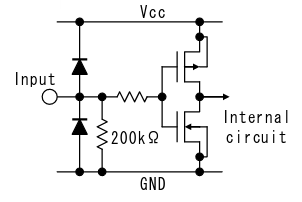
\includegraphics[width=0.4\textwidth,height=0.8\textheight,keepaspectratio]{figuras/ponteh.png}
 \caption{Diagrama de uma Ponte H \label{fig:ponte}}
 \vspace{-0.3cm}
 \caption*{\cite{pololu_motor}}.
\end{figure}


\begin{table}[h!]
\centering
 \captionsetup{width=0.5\textwidth,font=footnotesize,textfont=bf}
\caption{Especificações do \textit{driver} TB6612FNG da Toshiba \label{tab:ponteh}}
\begin{tabular}{llllllll}
\cline{1-2}
\bf Característica & \bf Descrição & & &  \\ \cline{1-2}
Tensão de alimentação & 15V & & &  \\
Corrente de saída & 1,2A  & & &  \\
Corrente de saída (pico) & 3,2A & & &  \\ \cline{1-2}
\end{tabular}
\caption*{\cite{pololu_motor} }
\end{table}


\vspace{0.5cm}
%%%%%%%%%%%%%%%%%%%%%%%%%%%%%%%%%%%%%%%%%%%%%%%%%%%%%%%%%%%%%%%%%%%%%%%%%%%%%%%%%%%%%%%%%%%%%%%%%%%%%%%%%%%%%%%
\section{Encoder magnético} \label{cap:encoder}

Um \textit{encoder} magnético é um transdutor de movimento, que converte movimentos em informações elétricas, %\cite{}.
sendo possível obter dados como posição e velocidade. Neste trabalho será utilizado o modelo 3081 da 
Pololu, %\textsuperscript{TM}, 
o qual pode ser visto na Figura \ref{fig:encoder}. Este dispositivo utiliza um disco 
magnético e sensor de efeito \textit{hall}, provendo doze contagens por revolução do eixo do motor \cite{pololu_encoder}. 

\begin{figure}[h!]
 \centering
 \captionsetup{width=0.4\textwidth,font=footnotesize,textfont=bf}
 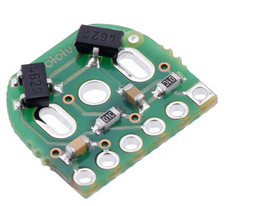
\includegraphics[width=0.4\textwidth,height=0.8\textheight,keepaspectratio]{figuras/encoder.png}
 \caption{Encoder magnético 3081 \label{fig:encoder}}
 \vspace{-0.3cm}
 \caption*{Fonte: \cite{pololu_encoder}}.
\end{figure}


\vspace{0.5cm}
%%%%%%%%%%%%%%%%%%%%%%%%%%%%%%%%%%%%%%%%%%%%%%%%%%%%%%%%%%%%%%%%%%%%%%%%%%%%%%%%%%%%%%%%%%%%%%%%%%%%%%%%%%%%%%%
\section{Sensores de refletância} \label{cap:reflet}
O sensor de refletância é um dispositivo eletrônico que consiste de um \textit{Light Emitter Diode} 
\sigla{LED}{\textit{Light Emitter Diode}} e um fototransistor, medindo assim a refletância de uma superfície. Este circuito, o 
pode ser visto na Figura \ref{fig:refletse}, 
será utilizado para detectar a linha do percurso. 
O modelo que será utilizado nesse trabalho é o QRE1113P, da Fairchild %\textsuperscript{TM} Semiconductor\cite{reflet}.
Semiconductor. 
As principais especificações deste dispositivo estão na Tabela \ref{tab:ref}.


\begin{figure}[h!]
 \centering
 \captionsetup{width=0.52\textwidth,font=footnotesize,textfont=bf}
 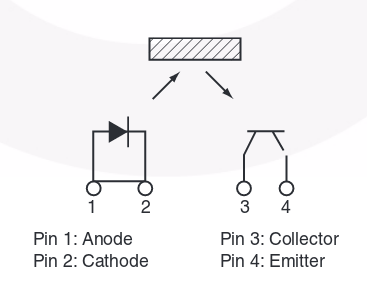
\includegraphics[width=0.5\textwidth,height=0.5\textheight,keepaspectratio]{figuras/qre.png}
 \caption{Motor HPCB 3041 \label{fig:refletse}}
 \vspace{-0.3cm}
 \caption*{Fonte: \cite{reflet}}.
\end{figure}


\begin{table}[h!]
\centering
 \captionsetup{width=0.47\textwidth,font=footnotesize,textfont=bf}
\caption{Especificações do sensor de refletância QRE1113P \label{tab:ref}}
\begin{tabular}{llllllll}
\cline{1-2}
\bf Característica & \bf Descrição & & &  \\ \cline{1-2}
Tensão de alimentação & 3,3V a 5V & & &  \\
Corrente de saída & 1,2A  & & &  \\
Corrente de saída (pico) & 3,2A & & &  \\ \cline{1-2}
\end{tabular}
\caption*{\cite{reflet}. }
\end{table}



\vspace{0.5cm}
%%%%%%%%%%%%%%%%%%%%%%%%%%%%%%%%%%%%%%%%%%%%%%%%%%%%%%%%%%%%%%%%%%%%%%%%%%%%%%%%%%%%%%%%%%%%%%%%%%%%%%%%%%%%%%%
\section{Placa de circuito impresso} \label{cap:chassi}

O \textit{chassi} do robô, ou seja, a estrutura deste, será confeccionada em uma placa de 
circuito impresso (\sigla{PCB}{\textit{Printed Circuit Board}}) de fenolite.



\vspace{0.5cm}
%%%%%%%%%%%%%%%%%%%%%%%%%%%%%%%%%%%%%%%%%%%%%%%%%%%%%%%%%%%%%%%%%%%%%%%%%%%%%%%%%%%%%%%%%%%%%%%%%%%%%%%%%%%%%%%
\section{Módulo bluetooth} \label{cap:bluetooth}\

Será utilizado o módulo \textit{bluetooth} %\textregistered 
HC-05 para a telemetria. Este módulo possuiu a configuração 
mestre-escravo e comunicação \textit{Universal Asynchronous Receiver Transmitter} 
(\sigla{UART}{\textit{Universal Asynchronous Receiver Transmitter}}).

\begin{figure}[h!]
 \centering
 \captionsetup{width=0.4\textwidth,font=footnotesize,textfont=bf}
 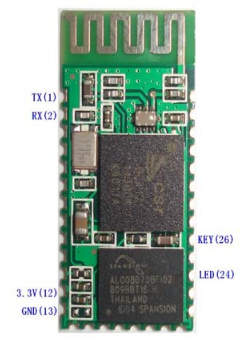
\includegraphics[width=0.4\textwidth,height=0.8\textheight,keepaspectratio]{figuras/hc05.png}
 \caption{Módulo \textit{bluetooth} HC-05 \label{fig:hc05}}
 \vspace{-0.3cm}
 \caption*{\cite{hc05}}.
\end{figure}



\vspace{0.5cm}
%%%%%%%%%%%%%%%%%%%%%%%%%%%%%%%%%%%%%%%%%%%%%%%%%%%%%%%%%%%%%%%%%%%%%%%%%%%%%%%%%%%%%%%%%%%%%%%%%%%%%%%%%%%%%%%
\section{Rodas e pneus} \label{cap:rodas}
Serão utilizadas rodas com pneus de poliuretano ou silicone. As rodas serão adquiridas ou, se possível, implementadas em 
impressora 3D.


\vspace{0.5cm}
%%%%%%%%%%%%%%%%%%%%%%%%%%%%%%%%%%%%%%%%%%%%%%%%%%%%%%%%%%%%%%%%%%%%%%%%%%%%%%%%%%%%%%%%%%%%%%%%%%%%%%%%%%%%%%%
\section{Bateria Lipo} \label{cap:bateria}

A alimentação do robô será feita por uma bateria do tipo Lítio-Polímero (\sigla{Li-Po}{Lítio-Polímero}) de duas céluas, 11,1V, 300mAh e 
32,5A de corrente máxima de descarga, pois possui alta capacidade de corrente e densidade de carga.
\vspace{0.5cm}

%%%%%%%%%%%%%%%%%%%%%%%%%%%%%%%%%%%%%%%%%%%%%%%%%%%%%%%%%%%%%%%%%%%%%%%%%%%%%%%%%%%%%%%%%%%%%%%%%%%%%%%%%%%%%%%
%\section{Conversor Step-Up} \label{cap:stepup}
%O conversor \textit{Step-up} que será utilizado é o XL6009, que é um módulo elevador de tensão. Este circuito possui 
%eficiência de 94\%, corrente e tensão de saída máxima de 3A e 35V, respectivamente \cite{stepup}.
%\vspace{0.5cm}


%\newline


%%%%%%%%%%%%%%%%%%%%%%%%%%%%%%%%%%%%%%%%%%%%%%%%%%%%%%%%%%%%%%%%%%%%%%%%%%%%%%%%%%%%%%%%%%%%%%%%%%%%%%%%%%%%%%%
%\section{Esfera deslizante} \label{cap:esfera}
%Será utilizada uma esfera deslizante para sustentar a parte frontal do robô e manter os sensores de refletância em sua 
%correta posição de funcionamento.
%\vspace{0.5cm}


%\newline


%%%%%%%%%%%%%%%%%%%%%%%%%%%%%%%%%%%%%%%%%%%%%%%%%%%%%%%%%%%%%%%%%%%%%%%%%%%%%%%%%%%%%%%%%%%%%%%%%%%%%%%%%%%%%%%
%\section{Step-Down} \label{cap:stepdown}

%\newline




% https://www.pololu.com/product/3038

% https://www.pololu.com/product/3081



